\documentclass[tikz,border=8pt]{standalone}
\usepackage{amsmath,amssymb}
\usetikzlibrary{arrows.meta,calc,decorations.pathmorphing}

\begin{document}
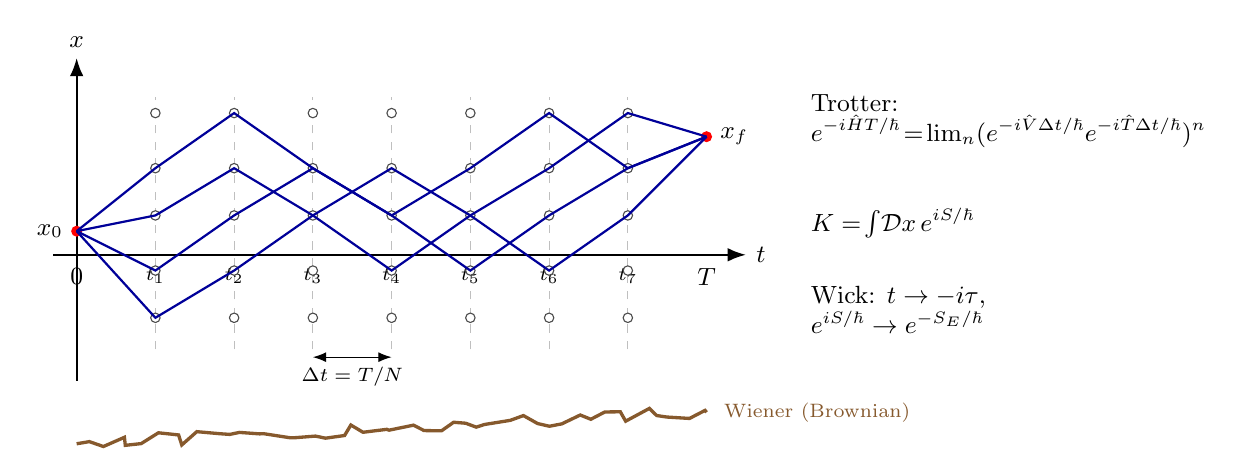
\begin{tikzpicture}[>=Latex]

  % axes
  \draw[->, thick] (-0.3, 0) -- (8.5, 0) node[right, font=\small]{$t$};
  \draw[->, thick] (0, -1.6) -- (0, 2.5) node[above, font=\small]{$x$};

  % time slices
  \foreach \k in {1,2,3,4,5,6,7}{
    \pgfmathsetmacro{\tx}{\k*1.0}
    \draw[gray!50, dashed] (\tx, -1.2) -- (\tx, 2.0);
    \node[font=\scriptsize, anchor=north] at (\tx, -0.05) {$t_\k$};
  }

  % Endpoints
  \fill[red] (0, 0.3) circle (0.07);
  \node[font=\small, anchor=east] at (-0.05, 0.3) {$x_0$};
  \fill[red] (8, 1.5) circle (0.07);
  \node[font=\small, anchor=west] at (8.05, 1.5) {$x_f$};

  % Open circles at intermediate slice points (insertions of complete basis)
  \foreach \tx in {1, 2, 3, 4, 5, 6, 7}{
    \foreach \y in {-0.8, -0.2, 0.5, 1.1, 1.8}{
      \draw[gray!60!black, fill=white, thin] (\tx, \y) circle (0.06);
    }
  }

  % Several broken-line paths
  \draw[blue!60!black, thick] (0, 0.3) -- (1, -0.2) -- (2, 0.5) -- (3, 1.1) -- (4, 0.5) -- (5, -0.2) -- (6, 0.5) -- (7, 1.1) -- (8, 1.5);
  \draw[blue!60!black, thick] (0, 0.3) -- (1, 1.1) -- (2, 1.8) -- (3, 1.1) -- (4, 0.5) -- (5, 1.1) -- (6, 1.8) -- (7, 1.1) -- (8, 1.5);
  \draw[blue!60!black, thick] (0, 0.3) -- (1, -0.8) -- (2, -0.2) -- (3, 0.5) -- (4, 1.1) -- (5, 0.5) -- (6, 1.1) -- (7, 1.8) -- (8, 1.5);
  \draw[blue!60!black, thick] (0, 0.3) -- (1, 0.5) -- (2, 1.1) -- (3, 0.5) -- (4, -0.2) -- (5, 0.5) -- (6, -0.2) -- (7, 0.5) -- (8, 1.5);

  % Δt indicator
  \draw[<->, thin] (3.0, -1.3) -- (4.0, -1.3);
  \node[font=\scriptsize, anchor=north] at (3.5, -1.3) {$\Delta t = T/N$};

  % Right side equations
  \node[font=\small, anchor=west, align=left] at (9.2, 1.7)
    {Trotter:\\$e^{-i\hat H T/\hbar}\!=\!\lim_n(e^{-i\hat V\Delta t/\hbar}e^{-i\hat T\Delta t/\hbar})^n$};
  \node[font=\small, anchor=west, align=left] at (9.2, 0.4)
    {$K=\!\int\!\mathcal D x\,e^{iS/\hbar}$};

  \node[font=\small, anchor=west, align=left] at (9.2, -0.7)
    {Wick: $t\to-i\tau$,\\$e^{iS/\hbar}\to e^{-S_E/\hbar}$};

  % Wiener path (jagged) at bottom
  \draw[brown!70!black, very thick, decorate, decoration={random steps, segment length=5pt, amplitude=2.5pt}]
    (0, -2.4) -- (8, -2.0);
  \node[font=\scriptsize, brown!70!black, anchor=west] at (8.1, -2.0) {Wiener (Brownian)};

  % T-axis bottom labels
  \node[font=\small, anchor=north] at (0, -0.05) {$0$};
  \node[font=\small, anchor=north] at (8, -0.05) {$T$};
\end{tikzpicture}
\end{document}
